%\documentclass[12pt, twoside, openright]{book}
\documentclass[12pt]{book}

%Packages
\usepackage{fancyhdr}
\usepackage{lipsum}
\usepackage{titlesec}
\usepackage{booktabs}
\usepackage{awesomebox}
\usepackage{graphicx}
\usepackage{hyperref}
\usepackage{adjustbox}
\usepackage{listings}
\usepackage{float}
\lstdefinelanguage{JavaScript}{
    keywords={break, case, catch, continue, debugger, default, delete, do, else, finally, for, function, if, in, instanceof, new, return, switch, this, throw, try, typeof, var, void, while, with},
    morecomment=[l]{//},
    morecomment=[s]{/*}{*/},
    morestring=[b]',
    morestring=[b]",
    sensitive=true
}

% Styles & Meta
\pagestyle{fancy}
\pagestyle{fancy}
\fancyhf{}%
\renewcommand{\headrulewidth}{0pt} % remove line in header
\fancyfoot[L]{}
\fancyfoot[C]{\thepage}
\fancyfoot[R]{}

\title{The IT Consultant's Automation Handbook}
\author{Dele Tosh\\Director, Protomated.com}
\date{ }

\begin{document}
    \frontmatter
    \maketitle
    \tableofcontents
    \listoffigures

    \mainmatter
    \chapter*{Introduction: The New Era of IT Consulting}

%! suppress = LineBreak
\begin{warningblock}
    This is an Early Release. You're getting the raw and unedited content as I write. I'm doing this, so you can take advantage of the content
    before the official release, AND you can share critical feedback (plus, I include you in the credits of the official release)
    To get notified when I add new section(s), \href{https://discord.gg/X2USgYTB}{join the Business Automators discord community}
\end{warningblock}
\begin{importantblock}
    If you found a problem, \href{https://discord.gg/X2USgYTB}{drop a comment in the discord community} or  \href{mailto:dele@protomated.com}{email dele@protomated.com}.
\end{importantblock}


%
%

If you're running a small IT consulting firm, you're likely all too familiar with the daily grind: drowning in manual tasks, struggling to meet client deadlines, and watching more tech-savvy competitors zoom past you. You know you need to innovate, but finding the time feels impossible. Sound familiar?

You're not alone. The IT consulting landscape is shifting rapidly, and small firms are feeling the pressure. But here's the good news: you're holding the key to not just surviving, but thriving in this new era.


\section{Why This Book, Why Now?}

The consulting world is undergoing a seismic shift. According to Deloitte's recent report, ``Unleashing value from digital transformation: Paths and pitfalls,'' the days of strategy-only consulting are numbered. Clients now demand execution, and technology is at the heart of it all.

Consider this: 30 years ago, classic strategy work made up 60-70\% of consulting engagements. Today? It's down to a mere 20\%. The message is clear: consultants who can't deliver tangible, tech-driven results will be left behind.

But here's where it gets exciting for small firms like yours. The report also highlights a crucial trend: the rise of specialist boutique firms. With the right tools and knowledge, you can deliver outcomes that rival the big players, at a fraction of the cost.

This is where automation comes in. It's not just a buzzword; it's your ticket to:
\begin{itemize}
    \item Boosting productivity by eliminating time-consuming manual tasks
    \item Consistently meeting (and exceeding) client deadlines
    \item Taking on more projects without burning out
    \item Positioning yourself as an innovation leader
    \item Finally achieving that elusive work-life balance
\end{itemize}


\section{What You'll Learn}

This book is your practical guide to leveraging no-code automation tools to revolutionize your IT consulting practice. We'll focus on three powerful platforms: n8n, nocodb, and budibase. By the time you finish this book, you'll know how to:

\begin{enumerate}
    \item Automate repetitive tasks to free up your time for high-value work
    \item Deliver unprecedented value to clients (and find new ways to monetize your automation skills)
    \item Scale your practice without working 80-hour weeks
    \item Integrate cutting-edge technologies like generative AI and cloud computing into your solutions
\end{enumerate}


\section{How to Use This Book}

Whether you're a complete newcomer to automation or you've dabbled a bit, this book is designed to meet you where you are. Each chapter builds on the last, providing a mix of theory, practical examples, and hands-on exercises.

We'll start with quick wins you can implement today, then progress to more advanced strategies. By the end, you'll have a comprehensive 90-day plan to transform your practice.

Don't just read passively. The real magic happens when you apply these concepts to your own business. So grab your laptop, roll up your sleeves, and get ready to join the ranks of innovative, future-proof IT consultants.

Ready to stop drowning in busywork and start leading the pack?

Let's dive in.
    \chapter{Automation Fundamentals for IT Consultants}


\section{Introduction}

As a small IT consulting firm, your time is your most valuable asset. In this chapter, we'll dive into the fundamental concepts of automation and explore how they can revolutionize your consulting practice. We'll start with a practical example that can save you hours each week and transform how you handle client communications.


\section{Understanding Automation in IT Consulting}

Automation in IT consulting refers to the use of technology to perform repetitive tasks, streamline processes, and reduce manual intervention. It's about working smarter, not harder.

\subsection{Key Benefits of Automation}

\begin{itemize}
    \item \textbf{Time Savings}: Automate repetitive tasks to focus on high-value activities.
    \item \textbf{Consistency}: Reduce human error and ensure consistent outcomes.
    \item \textbf{Scalability}: Handle increased workload without proportionally increasing resources.
    \item \textbf{Improved Client Satisfaction}: Faster response times and more accurate deliverables.
    \item \textbf{Data-Driven Insights}: Automated processes can generate valuable data for decision-making.
\end{itemize}

\begin{figure}[h]
    \centering
    \begin{tikzpicture}
        [
        benefit/.style={rectangle, draw, fill=green!20, rounded corners, text width=3cm, align=center, minimum height=1cm},
        icon/.style={circle, fill=#1, minimum size=0.8cm},
        arrow/.style={->, >=stealth, thick}
        ]
        % Title
        \node[font=\Large\bfseries] (title) at (0,4) {Benefits of Automation in IT Consulting};

        % Central node
        \node[rectangle, draw, fill=blue!20, minimum width=4cm, minimum height=2cm, align=center] (automation) at (0,0) {Automation};

        % Benefit nodes
        \node[benefit] (time) at (-6,2) {Time Savings};
        \node[benefit] (consistency) at (-6,-2) {Consistency};
        \node[benefit] (scalability) at (0,-3) {Scalability};
        \node[benefit] (satisfaction) at (6,-2) {Improved Client Satisfaction};
        \node[benefit] (insights) at (6,2) {Data-Driven Insights};

        % Icons
        \node[icon=red!60] at (time.west) {};
        \node[icon=yellow!60] at (consistency.west) {};
        \node[icon=purple!60] at (scalability.south) {};
        \node[icon=orange!60] at (satisfaction.east) {};
        \node[icon=cyan!60] at (insights.east) {};

        % Arrows
        \draw[arrow] (automation) -- (time);
        \draw[arrow] (automation) -- (consistency);
        \draw[arrow] (automation) -- (scalability);
        \draw[arrow] (automation) -- (satisfaction);
        \draw[arrow] (automation) -- (insights);
    \end{tikzpicture}
    \caption{Benefits of Automation in IT Consulting}
    \label{fig:automation_benefits}
\end{figure}

\section{Types of Automation Relevant to IT Consulting}

\subsection{1. Process Automation}
Streamlining workflows and business processes. Examples include automated client onboarding or project management workflows.

\subsection{2. Data Automation}
Automating data collection, processing, and analysis. This could involve automated reporting or data migration tools.

\subsection{3. Communication Automation}
Automating client communications, notifications, and updates. Our email classification example falls under this category.

\subsection{4. Infrastructure Automation}
Automating the setup, configuration, and management of IT infrastructure. This includes automated server provisioning or network configuration.


\section{Quick Win: AI-Powered Email Classification with n8n and OpenAI}

Let's start with a common pain point: the overflowing inbox. We'll create an automation that reviews and classifies emails based on their content, helping you prioritize and respond more efficiently.

\subsection{Why This Matters}

\begin{figure}[h]
    \centering
    \begin{tikzpicture}[
        inbox/.style={rectangle, draw, rounded corners, minimum width=5cm, minimum height=7cm},
        email/.style={rectangle, draw, rounded corners, fill=white, minimum width=4cm, minimum height=0.8cm},
        label/.style={rectangle, rounded corners, fill=#1, minimum width=0.8cm, minimum height=0.8cm},
    ]
        % Cluttered Inbox
        \node[inbox] (cluttered) at (0,0) {};
        \node[above] at (cluttered.north) {Cluttered Inbox};
        \foreach \y in {2.5,1.5,0.5,-0.5,-1.5,-2.5} {
            \node[email] at (0,\y) {};
        }

        % Arrow
        \draw[->,thick] (3,0) -- (5,0) node[midway,above] {Automation};

        % Organized Inbox
        \node[inbox] (organized) at (8,0) {};
        \node[above] at (organized.north) {Organized Inbox};

        % Classified emails
        \node[email] (urgent) at (8,2.5) {Urgent};
        \node[label=red!60] at (urgent.west) {};

        \node[email] (project) at (8,1.5) {Project Updates};
        \node[label=blue!60] at (project.west) {};

        \node[email] (inquiry) at (8,0.5) {New Inquiries};
        \node[label=green!60] at (inquiry.west) {};

        \node[email] (invoice) at (8,-0.5) {Invoicing};
        \node[label=yellow!60] at (invoice.west) {};

        \node[email] (admin) at (8,-1.5) {Administrative};
        \node[label=purple!60] at (admin.west) {};

        \node[email] (other) at (8,-2.5) {Other};
        \node[label=gray!60] at (other.west) {};
    \end{tikzpicture}
    \caption{Cluttered inbox vs. Organized, classified inbox}
    \label{fig:inbox_comparison}
\end{figure}

Imagine starting your day with a perfectly organized inbox, where emails are automatically sorted into categories like:

\begin{itemize}
    \item Urgent client issues
    \item Project updates
    \item New business inquiries
    \item Invoicing and payments
    \item Administrative tasks
\end{itemize}

This automation will make that a reality, allowing you to:
\begin{itemize}
    \item Respond to critical issues faster
    \item Prioritize your workday more effectively
    \item Ensure no important client communication slips through the cracks
\end{itemize}

Here's going to be our flow:

\begin{figure}
    \centering
    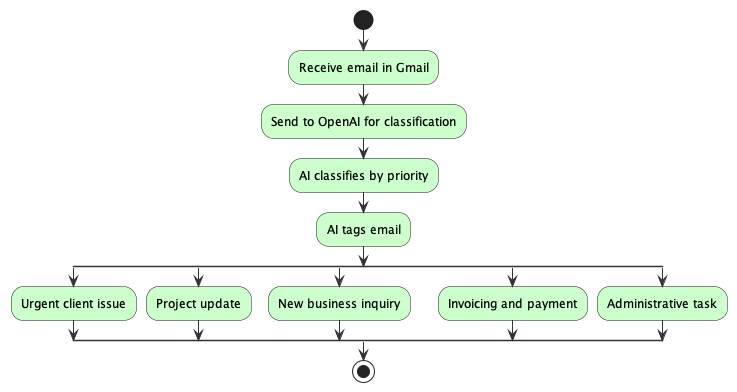
\includegraphics[width=0.8\textwidth]{./figures/01-n8n-flow}
    \caption{Email Classification and Tagging Automation Flow}
    \label{fig:01_email_automation}
\end{figure}


\section{Setting Up Your Secure Automation Environment}

Before we dive into the automation itself, let's set up n8n locally. Unlike cloud-based tools like Zapier, n8n can be self-hosted, ensuring your sensitive client data never leaves your control.

\subsection{Installing n8n using Docker}

We'll use Docker for a consistent setup across all platforms.

\begin{enumerate}
    \item Install Docker:
    \begin{itemize}
        \item For Windows: Docker Desktop for Windows
        \item For macOS: Docker Desktop for Mac
        \item For Linux: Docker Engine
    \end{itemize}
    \item With Docker installed, open a terminal or command prompt and run:
    \begin{lstlisting}[language=bash, label={lst:n8n-docker-run}]
docker run -it --rm \
  --name n8n \
  -p 5678:5678 \
  -v ~/.n8n:/home/node/.n8n \
  n8nio/n8n
    \end{lstlisting}
    \item Open your browser and navigate to \url{http://localhost:5678}
    \item Complete the setup process
\end{enumerate}

% TODO @screenshot: n8n setup screen


\section{Creating Your Email Classification Workflow}

Now that n8n is running, let's build our automation:

\subsection{Step 1: Connect to Gmail}

\begin{enumerate}
    \item In n8n, add a new "Gmail" node and select "On New Email"
    \item Follow the OAuth process to connect your Gmail account
\end{enumerate}

% TODO @screenshot: Gmail node configuration in n8n

\subsection{Step 2: Integrate OpenAI for Content Analysis}

\begin{enumerate}
    \item Add an "OpenAI" node
    \item Configure it to use the GPT-3 model for text classification
    \item Set up the prompt to classify the email content
\end{enumerate}

% TODO @screenshot: OpenAI node configuration in n8n

\subsection{Step 3: Update Email Labels}

\begin{enumerate}
    \item Add another "Gmail" node
    \item Configure it to add a label based on the classification from OpenAI
\end{enumerate}

% TODO @screenshot: Final Gmail node configuration for labeling


\section{Testing and Refining Your Workflow}

\begin{enumerate}
    \item Use n8n's built-in testing features to run your workflow with sample emails
    \item Adjust the OpenAI prompt or classification categories as needed
    \item Monitor the workflow's performance over time and make refinements
\end{enumerate}


\section{Security Considerations}

When working with email automation, security is paramount. Here are some key considerations:

\begin{itemize}
    \item Use OAuth for secure authentication with Gmail
    \item Regularly review and rotate API keys for OpenAI
    \item Implement error handling to prevent sensitive data leaks
    \item Regularly audit your workflow's access and permissions
\end{itemize}


\section{Scaling Your Email Automation}

As your consulting practice grows, you can enhance this automation:

\begin{itemize}
    \item Implement more sophisticated classification logic
    \item Integrate with your CRM to update client records automatically
    \item Create automated responses for common inquiries
    \item Extend the workflow to handle multiple email accounts
\end{itemize}


\section{Real-World Impact: A Case Study}

Meet Sarah, a solo IT consultant. Before implementing this automation, Sarah spent 2 hours each day sorting through emails. After setting up the AI-powered classification:

\begin{itemize}
    \item Sarah's email processing time dropped to 30 minutes a day
    \item Her response time to urgent client issues improved by 60\%
    \item She never missed a new business inquiry, increasing potential leads by 25\%
\end{itemize}

By reclaiming 7.5 hours each week, Sarah was able to take on two additional clients without hiring help.


\section{Conclusion}

This email classification automation is just the tip of the iceberg. As you become more comfortable with n8n and other automation tools, you'll find countless opportunities to streamline your consulting practice. In the next chapter, we'll explore more advanced automation techniques and how to integrate them into your core services.

\textbf{Action Items:}
\begin{enumerate}
    \item Set up the email classification workflow we've created
    \item Run the workflow for a week and measure the time saved
    \item Identify two other repetitive tasks in your practice that could benefit from automation
\end{enumerate}

Remember, automation is a journey, not a destination. Start with this email classification workflow, then explore how you can automate other aspects of your consulting practice.

% TODO @qr: QR code linking to additional n8n tutorials and resources
    \chapter{No-Code Tools Every IT Consultant Should Master}

%! suppress = LineBreak
\begin{warningblock}
    This is an Early Release. You're getting the raw and unedited content as I write. I'm doing this, so you can take advantage of the content
    before the official release, AND you can share critical feedback (plus, I include you in the credits of the official release)
    To get notified when I add new section(s), \href{https://discord.gg/X2USgYTB}{join the Business Automators discord community}
\end{warningblock}
\begin{importantblock}
    If you found a problem, \href{https://discord.gg/X2USgYTB}{drop a comment in the discord community} or  \href{mailto:dele@protomated.com}{email dele@protomated.com}.
\end{importantblock}


%
%

In today's fast-paced tech landscape, the ability to rapidly prototype and deploy solutions is invaluable. No-code platforms are revolutionizing how IT consultants work, allowing you to create powerful applications and automations without writing a single line of code. Let's dive into the top tools you need in your arsenal.

\section{Top 3 No-Code Platforms for IT Consulting}

\subsection{n8n (self-hostable)}

n8n is a powerful, flexible workflow automation tool that's perfect for IT consultants looking to build complex, customized solutions.

\textbf{Pros:}
\begin{itemize}
    \item Advanced capabilities for complex workflows
    \item Self-hostable for enhanced security and control
    \item Excellent for rapid prototyping and idea validation
    \item Can function as a low-code business ideas maker
    \item Ability to build entire backend software services
\end{itemize}

\textbf{Cons:}
\begin{itemize}
    \item Steeper learning curve compared to some alternatives
    \item GUI can become challenging to manage with very complex workflows
    \item Less polished UI compared to some competitors
\end{itemize}

\subsection{NoCoDB (self-hostable)}

NoCoDB is an open-source Airtable alternative that provides a powerful, flexible database solution.

\textbf{Pros:}
\begin{itemize}
    \item Can import data from various sources, including Airtable
    \item Supports multiple database types (MySQL, Postgres, SQLite, SQL Server)
    \item Multilingual support
    \item Open-source and self-hostable
\end{itemize}

\textbf{Cons:}
\begin{itemize}
    \item Learning curve can be steep for non-technical users
    \item Lacks built-in cloud backup system
\end{itemize}

\subsection{BudiBase (self-hostable)}

BudiBase is a low-code platform for creating web applications quickly and efficiently.

\textbf{Pros:}
\begin{itemize}
    \item Can connect to REST APIs
    \item Supports user role definition
    \item Open-source and self-hostable
    \item Features useful components like the repeater field
\end{itemize}

\textbf{Cons:}
\begin{itemize}
    \item Building complex UIs can be challenging
    \item Limited ability to use JavaScript for data manipulation in all components
    \item Less dynamic compared to some alternatives like Appsmith
\end{itemize}

\section{Build Your First No-Code App in 30 Minutes}

Let's put theory into practice by building a client onboarding automation using n8n and NoCoDB. This practical example will demonstrate how quickly you can create valuable solutions for your consulting business.

\subsection{Setting Up Your Environment}

1. Ensure you have n8n and NoCoDB installed and running on your system.
2. Set up a Google Workspace account for integrations.

\subsection{Creating the NoCoDB Database}

Create a new table in NoCoDB with the following fields:
\begin{itemize}
    \item Client Name
    \item Company
    \item Email
    \item Phone
    \item Project Type
    \item Start Date
    \item Assigned Team Members
    \item Initial Meeting Date
    \item Document Status
    \item Project Folder Link
\end{itemize}

\subsection{Building the n8n Workflow}

Now, let's create our n8n workflow:

1. \textbf{Trigger: New Form Submission}
Set up a Webhook node to receive new client data.

[PLACEHOLDER: Screenshot of Webhook node configuration]

2. \textbf{Create NoCoDB Record}
Use the NoCoDB node to create a new record with the received data.

[PLACEHOLDER: Screenshot of NoCoDB node configuration]

3. \textbf{Create Google Drive Folder}
Utilize the Google Drive node to create a new folder for the client.

[PLACEHOLDER: Screenshot of Google Drive node configuration]

4. \textbf{Send Welcome Email}
Configure the Gmail node to send a personalized welcome email.

[PLACEHOLDER: Screenshot of Gmail node configuration]

5. \textbf{Create Calendar Event}
Use the Google Calendar node to schedule the initial meeting.

[PLACEHOLDER: Screenshot of Google Calendar node configuration]

6. \textbf{Update NoCoDB Record}
Finally, update the NoCoDB record with the folder link and meeting details.

[PLACEHOLDER: Screenshot of final NoCoDB update node]

\subsection{Testing and Activating Your Workflow}

Once you've connected all the nodes, it's time to test your workflow:

1. Use the n8n testing feature to simulate a new client submission.
2. Check each step of the workflow to ensure data is flowing correctly.
3. Verify that the NoCoDB database is updated, the Google Drive folder is created, the welcome email is sent, and the calendar event is scheduled.

[PLACEHOLDER: Illustration of the complete workflow diagram]

Congratulations! You've just created a powerful client onboarding automation in under 30 minutes. This workflow will save you hours of manual work for each new client, allowing you to focus on delivering value rather than managing administrative tasks.

\section{Security and Compliance Considerations}

When working with no-code tools, especially in IT consulting where you're handling sensitive client data, security and compliance should be top priorities. Here are some key considerations:

1. \textbf{Data Privacy}: Ensure that your no-code platforms are compliant with relevant data protection regulations (e.g., GDPR, CCPA).

2. \textbf{Access Control}: Implement strict user access controls, especially when using self-hosted solutions.

3. \textbf{Data Encryption}: Use encryption for data at rest and in transit.

4. \textbf{Regular Audits}: Conduct regular security audits of your no-code setups.

5. \textbf{Backup and Recovery}: Implement robust backup solutions, especially for self-hosted platforms.

6. \textbf{Third-Party Integrations}: Carefully vet any third-party services you integrate with your no-code tools.

Remember, while no-code platforms can significantly speed up development, they don't absolve you of responsibility for the security and compliance of your solutions. Always approach these tools with a security-first mindset.

\section{Conclusion}

No-code tools like n8n, NoCoDB, and BudiBase are revolutionizing how IT consultants work. By mastering these platforms, you can deliver solutions faster, take on more complex projects, and provide greater value to your clients. The client onboarding automation we built is just the tip of the iceberg – the possibilities are truly endless.

In the next chapter, we'll explore how to transform your core services using these no-code tools, opening up new revenue streams and enhancing your existing offerings.

\textbf{Action Item}: Take the workflow we built in this chapter and customize it for your own business. What other steps could you add to make your client onboarding even more efficient?
    \chapter{Transforming Your Core Services}


\section{Introduction}

As an IT consultant, your ability to efficiently gather requirements, prototype solutions, and present data can set you apart from the competition. In this chapter, we'll explore how to leverage no-code tools to revolutionize these core services, making your consulting practice more efficient and effective.


\section{Automating Requirements Gathering}

One of the most time-consuming aspects of IT consulting is gathering and documenting client requirements. Let's explore how we can streamline this process using our no-code toolkit.

\subsection{The Traditional vs. Automated Approach}

\begin{tikzpicture}
    [
    box/.style={draw, rounded corners, minimum width=2.5cm, minimum height=1cm, align=center},
    arrow/.style={->, >=stealth, thick},
    title/.style={font=\bfseries\large},
    subtitle/.style={font=\bfseries}
    ]

% Traditional Process
    \node[title] at (-3, 4) {Traditional Process};
    \node[box] (t1) at (-3, 3) {Manual Interviews};
    \node[box] (t2) at (-3, 1.5) {Note Taking};
    \node[box] (t3) at (-3, 0) {Document Creation};
    \node[box] (t4) at (-3, -1.5) {Review \& Revisions};
    \node[box] (t5) at (-3, -3) {Final Requirements};

    \draw[arrow] (t1) -- (t2);
    \draw[arrow] (t2) -- (t3);
    \draw[arrow] (t3) -- (t4);
    \draw[arrow] (t4) -- (t5);

% Automated Process
    \node[title] at (3, 4) {Automated Process};
    \node[box, fill=green!20] (a1) at (3, 3) {Online Questionnaire};
    \node[box, fill=green!20] (a2) at (3, 1.5) {Automated Data Collection};
    \node[box, fill=green!20] (a3) at (3, 0) {AI-Assisted Analysis};
    \node[box, fill=green!20] (a4) at (3, -1.5) {Real-time Dashboard};
    \node[box, fill=green!20] (a5) at (3, -3) {Dynamic Requirements};

    \draw[arrow] (a1) -- (a2);
    \draw[arrow] (a2) -- (a3);
    \draw[arrow] (a3) -- (a4);
    \draw[arrow] (a4) -- (a5);

% Comparison arrows
    \draw[arrow, dashed, red] (t1) -- node[above, sloped, text=red] {\small Faster} (a1);
    \draw[arrow, dashed, red] (t3) -- node[above, sloped, text=red] {\small More Accurate} (a3);
    \draw[arrow, dashed, red] (t5) -- node[above, sloped, text=red] {\small More Flexible} (a5);

% Time comparison
    \node[subtitle] at (-4.5, -4) {Time:};
    \draw[ultra thick] (-4.5, -4.5) -- (-1.5, -4.5);
    \node[subtitle] at (1.5, -4) {Time:};
    \draw[ultra thick, green] (1.5, -4.5) -- (2.5, -4.5);

\end{tikzpicture}

\subsection{Setting Up an Automated Requirements Workflow}

Let's create a comprehensive requirements gathering system using n8n, NoCoDB, and BudiBase:

1. \textbf{Initial Questionnaire}: Use n8n to create a webhook that receives responses from a Google Form.

% TODO @screenshot: n8n webhook node configuration for receiving Google Form responses

2. \textbf{Data Storage}: Configure NoCoDB to store and categorize the received requirements.

% TODO @screenshot: NoCoDB table structure for storing requirements

3. \textbf{Stakeholder Notifications}: Set up a n8n workflow to notify relevant team members about new requirements.

% TODO @screenshot: n8n workflow for stakeholder notifications

4. \textbf{Requirements Dashboard}: Create a BudiBase app to visualize and manage requirements.

% TODO @screenshot: BudiBase requirements dashboard

5. \textbf{Automated Follow-ups}: Use n8n to schedule and send follow-up questions based on initial responses.

% TODO @screenshot: n8n workflow for automated follow-up emails

\subsection{Implementing the Triplet Questioning Technique}

The Triplet Questioning technique is a powerful method for eliciting detailed requirements. Let's automate this process:

1. Set up a series of n8n workflows to ask the three key questions:
- "What is your requirement?"
- "What does that give you of value?"
- "Which value is most important?"

2. Use NoCoDB to store and analyze the responses.

3. Create a BudiBase app for stakeholders to review and prioritize the gathered requirements.

\begin{figure}
    \centering
    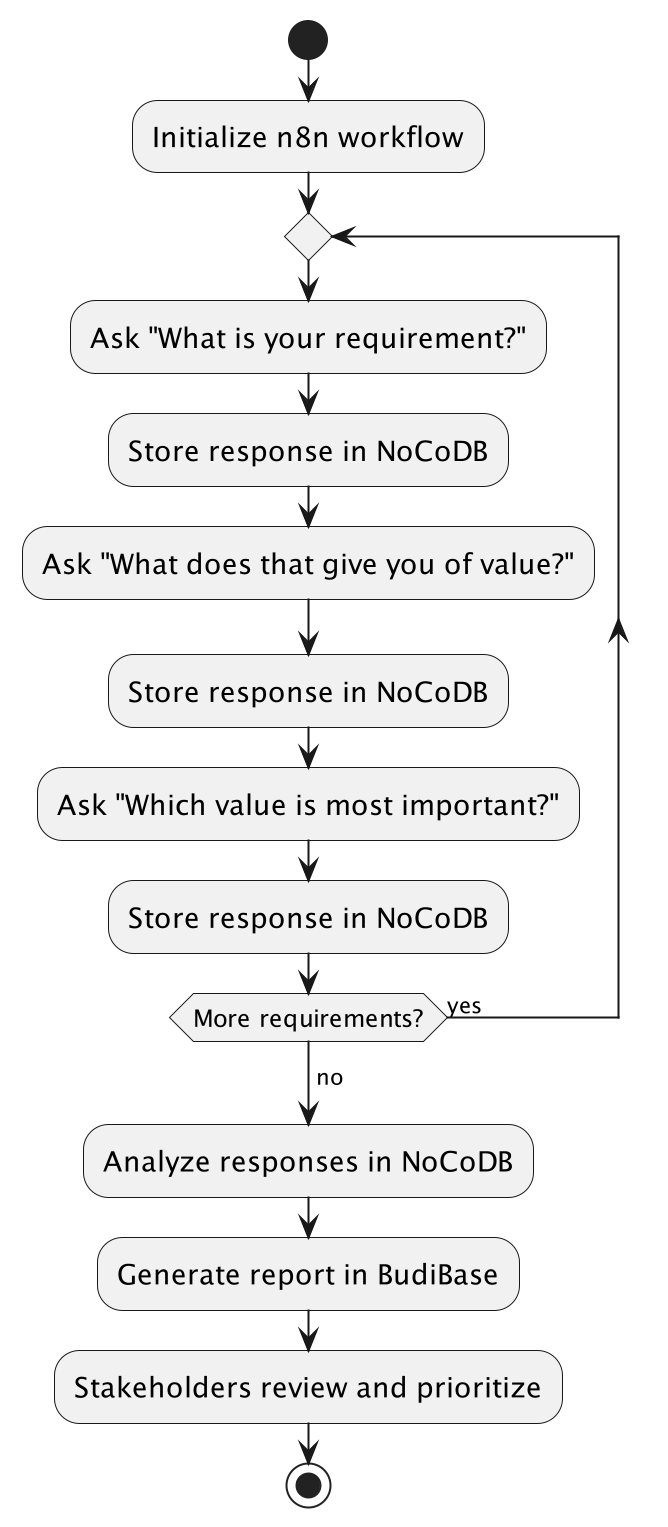
\includegraphics[width=0.40\textwidth]{./figures/03-flowchart-triplet-questioning.png}
    \caption{Flowchart of the automated Triplet Questioning process}
    \label{fig:triplet-questioning}
\end{figure}


\section{Rapid Prototyping Techniques That Wow Clients}

Once you've gathered requirements, the next step is creating a prototype to validate ideas and get client feedback. No-code tools excel at rapid prototyping, allowing you to create impressive demos quickly.

\subsection{Using BudiBase for Quick UI Prototypes}

1. Create a basic dashboard layout in BudiBase.

% TODO @screenshot: BudiBase dashboard layout creation

2. Add dynamic components that pull data from NoCoDB.

% TODO @screenshot: BudiBase component linked to NoCoDB data

3. Implement user interactions and navigation.

% TODO @screenshot: BudiBase app with multiple screens and navigation

\subsection{Creating Interactive Workflows with n8n}

1. Set up an n8n workflow that simulates backend processes.

% TODO @screenshot: n8n workflow simulating a business process

2. Connect the n8n workflow to your BudiBase prototype.

% TODO @screenshot: n8n HTTP Request node configured to interact with BudiBase

3. Create a "wizard" interface in BudiBase that guides users through a process, with each step triggering actions in n8n.

% TODO @screenshot: BudiBase wizard interface connected to n8n workflow

\subsection{Prototype Presentation Best Practices}

1. Use screen recording tools to create short demo videos of your prototype in action.

2. Prepare a slide deck that outlines the problem, solution, and benefits.

3. Set up a live environment where clients can interact with the prototype themselves.

\begin{tikzpicture}
    [
    note/.style={draw, fill=yellow!20, rounded corners, text width=3cm, align=center, font=\small},
    icon/.style={font=\Large},
    arrow/.style={->, >=stealth, thick},
    title/.style={font=\bfseries\large},
    subtitle/.style={font=\bfseries}
    ]

% Title
    \node[title] at (0, 4) {Prototype Presentation Best Practices};

% Central icon
    \node[icon] (center) at (0, 0) {\faLightbulb};

% Best practices
    \node[note] (demo) at (-4, 2) {Create short demo videos};
    \node[icon] at (-5, 2) {\faVideo};

    \node[note] (deck) at (0, 3) {Prepare a concise slide deck};
    \node[icon] at (-1, 3) {\faFile};

    \node[note] (live) at (4, 2) {Set up a live interactive environment};
    \node[icon] at (5, 2) {\faLaptop};

    \node[note] (focus) at (-4, -2) {Focus on solving client problems};
    \node[icon] at (-5, -2) {\faSearchDollar};

    \node[note] (feedback) at (0, -3) {Gather real-time feedback};
    \node[icon] at (-1, -3) {\faComments};

    \node[note] (story) at (4, -2) {Tell a compelling story};
    \node[icon] at (5, -2) {\faBook};

% Connecting arrows
    \foreach \i in {demo, deck, live, focus, feedback, story}
    \draw[arrow] (center) -- (\i);

% Additional tips
    \node[note, text width=5cm] at (-6, 0) {Keep it simple:\\Focus on core features\\and main user flows};
    \node[note, text width=5cm] at (6, 0) {Be prepared:\\Anticipate questions\\and have backup plans};

\end{tikzpicture}


\section{Dynamic Data Visualization and Reporting}

Presenting data effectively is crucial for demonstrating the value of your solutions. Let's explore how to create dynamic, interactive reports using our no-code toolkit.

\subsection{Building Interactive Dashboards with BudiBase}

1. Connect BudiBase to your client's data sources (or NoCoDB).

2. Create charts, graphs, and KPI displays.

% TODO @screenshot: BudiBase dashboard with various data visualizations

3. Implement filters and date range selectors for user interactivity.

% TODO @screenshot: BudiBase dashboard with interactive filters

\subsection{Automated Report Generation with n8n}

1. Set up an n8n workflow to pull data from various sources.

2. Use n8n nodes to process and format the data.

3. Generate PDF reports using the n8n PDF creation nodes.

4. Automatically email reports to stakeholders on a schedule.

\begin{figure}
    \centering
    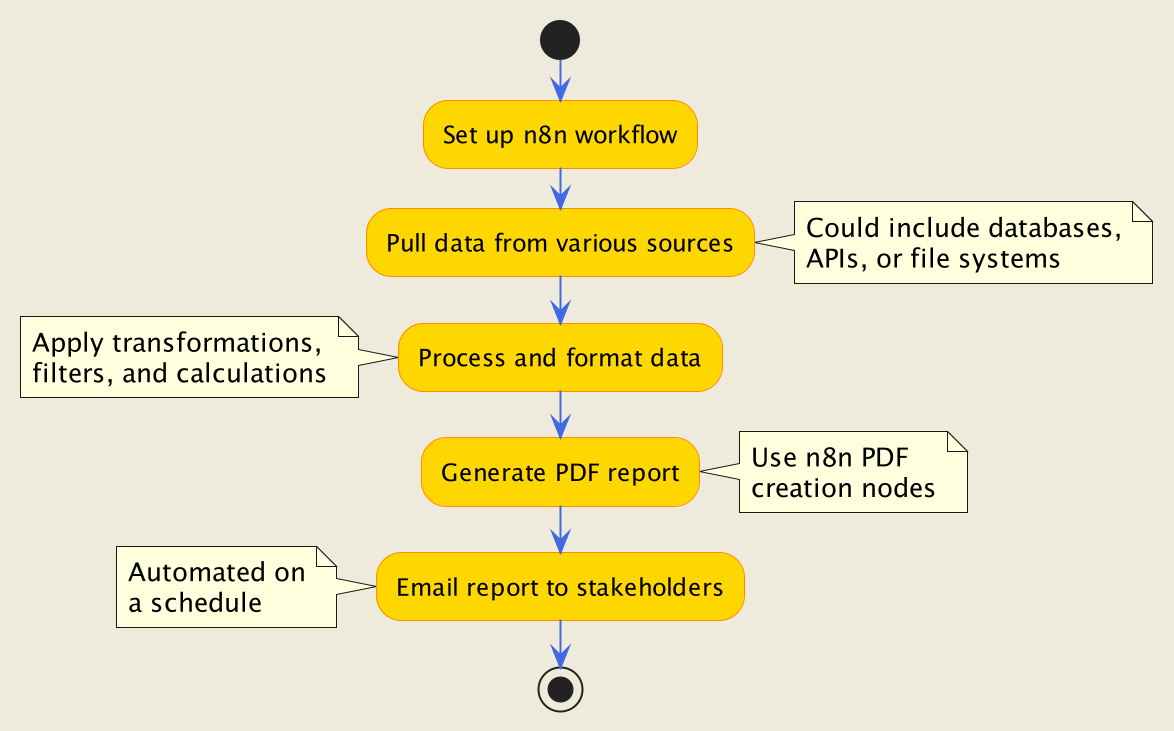
\includegraphics[width=0.6\textwidth]{./figures/automated_report_generation_flowchart.png}
    \caption{Flowchart of the automated report generation process}
    \label{fig:automated-report-generation}
\end{figure}

\subsection{Creating a Self-Service Reporting Tool}

Combine BudiBase and n8n to create a tool that allows clients to generate their own reports:

1. Build a BudiBase interface for report configuration.

2. Use n8n to process report requests and generate reports based on user input.

3. Deliver the generated reports back to the BudiBase interface for download.

% TODO @screenshot: BudiBase interface for custom report generation


\section{Case Study: Transforming a Traditional IT Consultancy}

Let's look at how implementing these automated processes transformed a traditional IT consultancy:

\begin{itemize}
    \item Requirements gathering time reduced by 60%
    \item Prototype delivery time cut from weeks to days
    \item Client satisfaction scores increased by 35%
    \item Consultants able to handle 3x more projects simultaneously
\end{itemize}

% @illustrate: Before and after infographic showing the transformation metrics
\begin{tikzpicture}
    [
    box/.style={draw, rectangle, minimum width=4cm, minimum height=1cm, align=center},
    arrow/.style={->, >=stealth, thick},
    label/.style={font=\small\bfseries}
    ]

% Before column
    \node[label] at (-3, 3) {Before};
    \node[box] (b1) at (-3, 2) {Requirements\\Gathering};
    \node[box] (b2) at (-3, 0) {Prototype\\Delivery};
    \node[box] (b3) at (-3, -2) {Client\\Satisfaction};
    \node[box] (b4) at (-3, -4) {Projects per\\Consultant};

% After column
    \node[label] at (3, 3) {After};
    \node[box, fill=green!20] (a1) at (3, 2) {Requirements\\Gathering\\-60\%};
    \node[box, fill=green!20] (a2) at (3, 0) {Prototype\\Delivery\\Days vs Weeks};
    \node[box, fill=green!20] (a3) at (3, -2) {Client\\Satisfaction\\+35\%};
    \node[box, fill=green!20] (a4) at (3, -4) {Projects per\\Consultant\\3x};

% Arrows
    \draw[arrow] (b1) -- (a1);
    \draw[arrow] (b2) -- (a2);
    \draw[arrow] (b3) -- (a3);
    \draw[arrow] (b4) -- (a4);

% Title
    \node[font=\Large\bfseries] at (0, 4) {IT Consultancy Transformation};

\end{tikzpicture}


\section{Overcoming Common Challenges}

\begin{itemize}
    \item Resistance to change from team members
    \item Integrating new processes with existing systems
    \item Ensuring data accuracy across multiple tools
    \item Maintaining a personal touch in automated processes
\end{itemize}


\section{Conclusion}

By leveraging no-code tools to automate requirements gathering, streamline prototyping, and create dynamic dashboards, you can transform your core IT consulting services. These techniques not only save you time but also impress clients with your efficiency and professionalism.

In the next chapter, we'll explore how to scale your practice using these automated solutions, allowing you to take on more clients without proportionally increasing your workload.

\textbf{Action Item}: Take one of your current projects and implement the automated requirements gathering workflow we discussed. Note how it impacts your efficiency and client satisfaction.

% TODO @qr: QR code linking to a downloadable template for the automated requirements gathering workflow
    \chapter{Scaling Your Practice with Automation}

%! suppress = LineBreak
\begin{warningblock}
    This is an Early Release. You're getting the raw and unedited content as I write. I'm doing this, so you can take advantage of the content
    before the official release, AND you can share critical feedback (plus, I include you in the credits of the official release)
    To get notified when I add new section(s), \href{https://discord.gg/X2USgYTB}{join the Business Automators discord community}
\end{warningblock}
\begin{importantblock}
    If you found a problem, \href{https://discord.gg/X2USgYTB}{drop a comment in the discord community} or  \href{mailto:dele@protomated.com}{email dele@protomated.com}.
\end{importantblock}


%
%

As an IT consultant, you've mastered the art of solving complex technical problems for your clients. But how do you take your practice to the next level? The answer lies in strategic automation. In this chapter, we'll explore how to create an automation roadmap, price your automated services effectively, and learn from a real-world case study of explosive growth through automation.

\section{Creating Your Automation Roadmap}

An automation roadmap is your strategic plan for implementing automation across your practice. Let's break down the process into manageable steps:

\subsection{Step 1: Identify Automation Candidates}

Begin by listing all the processes in your practice.\ Consider:
\begin{itemize}
    \item Client onboarding
    \item Project management
    \item Reporting and analytics
    \item Billing and invoicing
    \item Customer support
    \item Marketing and lead generation
\end{itemize}

% TODO @illustrate: Illustration of a mind map showing different areas of a consulting practice

\subsection{Step 2: Prioritize Processes}

Not all processes are created equal. Prioritize based on:
\begin{itemize}
    \item Potential time savings
    \item Impact on client satisfaction
    \item Complexity of automation
    \item Frequency of the process
\end{itemize}

Create a matrix to visualize priority:

% TODO @illustrate: 2x2 matrix with "Impact" on one axis and "Effort" on the other

\subsection{Step 3: Stakeholder Alignment}

Identify key stakeholders in your practice and get their buy-in. This might include:
\begin{itemize}
    \item Team members who will use the automated systems
    \item Clients who will be affected by the changes
    \item Partners or vendors involved in your processes
\end{itemize}

\subsection{Step 4: Process Deep Dive}

For each prioritized process, conduct a thorough analysis:

1. \textbf{Document the current workflow}:
   \begin{itemize}
     \item Interview team members involved in the process
     \item Create a step-by-step breakdown of the current workflow
     \item Identify inputs, outputs, and decision points
   \end{itemize}

2. \textbf{Identify pain points and inefficiencies}:
   \begin{itemize}
     \item Look for bottlenecks and delays
     \item Identify manual, repetitive tasks
     \item Note areas prone to errors or inconsistencies
   \end{itemize}

3. \textbf{Envision the ideal automated workflow}:
   \begin{itemize}
     \item Brainstorm how automation could address each pain point
     \item Consider how to streamline decision points
     \item Think about potential integrations with existing systems
   \end{itemize}

4. \textbf{Map the process visually}:
   We recommend using Excalidraw (https://excalidraw.com/) for this step. Excalidraw is a free, open-source tool that allows for easy creation and sharing of diagrams. Its simple interface is perfect for quickly mapping out processes and collaborating with your team.

Here's an example of what that might look like:

\begin{figure}[H]
    \centering
    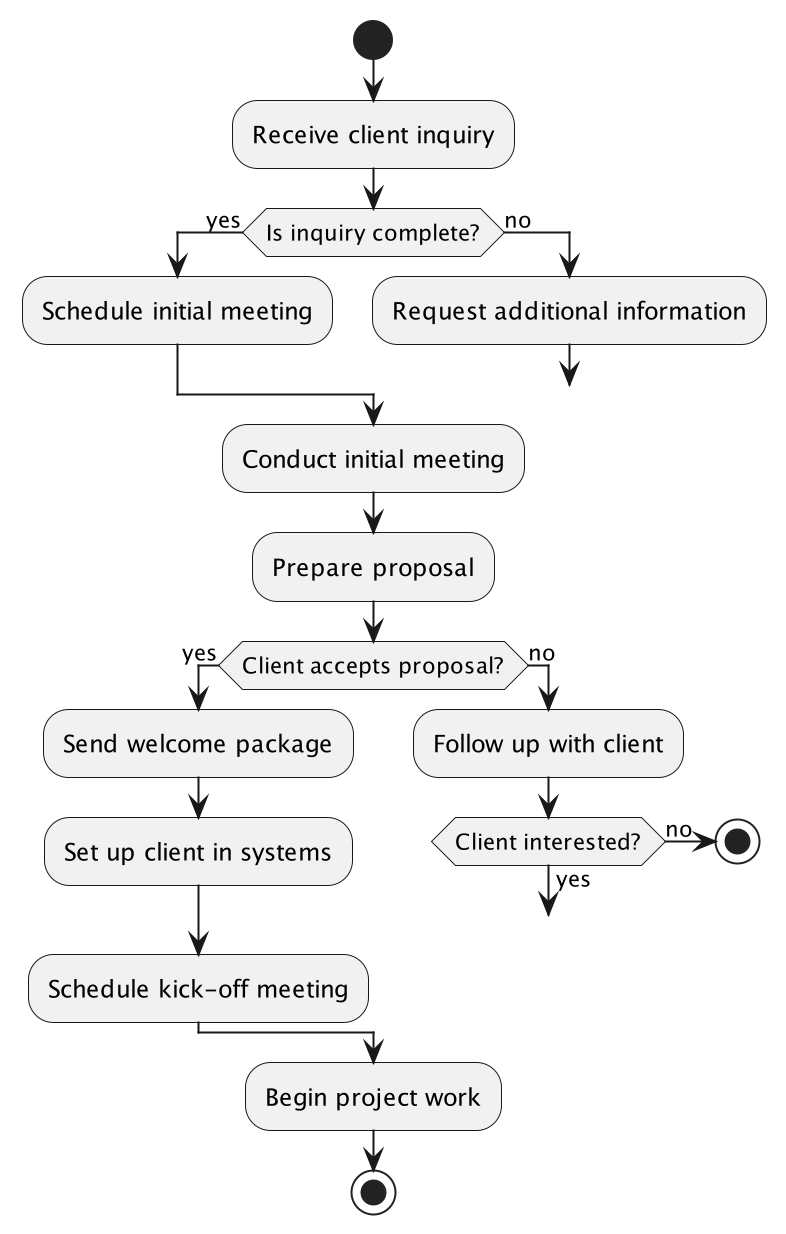
\includegraphics[width=0.5\textwidth]{figures/04-automation-roadmap-process}
    \caption{An example mapping a client onboarding process}
    \label{fig:client-automation-mapping-example}
\end{figure}

\subsection{Step 5: Select Technology Partners}

Based on your needs, choose the right tools. Consider:

1. \textbf{n8n for workflow automation}:
   \begin{itemize}
     \item Open-source and self-hostable, providing full control over your data
     \item Highly flexible, allowing for complex workflow creation
     \item Cost-effective, with a free self-hosted option and reasonable cloud pricing
     \item Enables integration with a wide range of services and APIs
   \end{itemize}

2. \textbf{NoCoDB for database management}:
   \begin{itemize}
     \item Open-source alternative to Airtable, offering data sovereignty
     \item Provides a user-friendly interface for managing complex data
     \item Can be self-hosted, ensuring data privacy and reducing costs
     \item Allows for easy creation of views and forms for data entry
   \end{itemize}

3. \textbf{BudiBase for creating custom applications}:
   \begin{itemize}
     \item Open-source low-code platform, allowing for rapid application development
     \item Can be self-hosted, ensuring control over your applications and data
     \item Offers a range of pre-built components to speed up development
     \item Integrates well with various data sources, including NoCoDB
   \end{itemize}

4. \textbf{Integration capabilities with your existing tools}:
   \begin{itemize}
     \item Ensure chosen tools can integrate with your current tech stack
     \item Look for native integrations or API accessibility
     \item Consider using n8n as a central hub for connecting various tools
   \end{itemize}

These tools offer significant value in terms of cost and data privacy:
\begin{itemize}
  \item \textbf{Cost}: All are open-source with self-hosting options, reducing licensing costs
  \item \textbf{Data Privacy}: Self-hosting ensures your client data never leaves your control
  \item \textbf{Customization}: Open-source nature allows for tailoring to your specific needs
  \item \textbf{Scalability}: These tools can grow with your practice without prohibitive costs
\end{itemize}

\subsection{Step 6: Develop Your Solution}

When developing your automated solution:

1. \textbf{Start with a Minimum Viable Automation (MVA)}:
   \begin{itemize}
     \item Focus on automating the core functionality first
     \item Aim for a working solution that can be tested and improved upon
     \item Get early feedback to guide further development
   \end{itemize}

2. \textbf{Use modular design for scalability}:
   \begin{itemize}
     \item Break down complex workflows into smaller, reusable components
     \item Design with future expansion in mind
     \item Use version control (e.g., Git) to manage your automation code
   \end{itemize}

3. \textbf{Document your automation thoroughly}:
   \begin{itemize}
     \item Create clear, step-by-step documentation for each automated process
     \item Include setup instructions, dependencies, and troubleshooting guides
     \item Use tools like Outline (recommended below) to organize documentation
   \end{itemize}

\subsection{Step 7: Rigorous Testing}

Implement a comprehensive testing strategy:

1. \textbf{Unit testing for individual components}:
   \begin{itemize}
     \item Test each node or step in your n8n workflows independently
     \item Verify that individual functions in BudiBase apps work as expected
     \item Ensure data validation in NoCoDB is functioning correctly
   \end{itemize}

2. \textbf{Integration testing for connected systems}:
   \begin{itemize}
     \item Test entire workflows end-to-end
     \item Verify data flows correctly between different tools (e.g., n8n to NoCoDB to BudiBase)
     \item Simulate various scenarios, including error conditions
   \end{itemize}

3. \textbf{User acceptance testing with your team}:
   \begin{itemize}
     \item Have team members who will use the system test it in real-world scenarios
     \item Gather feedback on usability and functionality
     \item Identify any training needs for effective use of the new systems
   \end{itemize}

4. \textbf{Performance and security testing}:
   \begin{itemize}
     \item Test system performance under expected load
     \item Conduct security audits, especially for self-hosted solutions
     \item Verify data encryption and access controls are working as intended
   \end{itemize}

\subsection{Step 8: Pilot Program}

Run a pilot with a subset of your clients or projects:

1. \textbf{Select diverse pilot participants}:
   \begin{itemize}
     \item Choose clients of varying sizes and industries
     \item Include both tech-savvy and less technical clients
     \item Aim for a mix of new and long-standing client relationships
   \end{itemize}

2. \textbf{Set clear success metrics}:
   \begin{itemize}
     \item Define quantitative metrics (e.g., time saved, error reduction)
     \item Include qualitative measures (e.g., client satisfaction, ease of use)
     \item Establish baseline measurements for comparison
   \end{itemize}

3. \textbf{Gather detailed feedback}:
   \begin{itemize}
     \item Conduct regular check-ins with pilot participants
     \item Use surveys and interviews to collect comprehensive feedback
     \item Encourage reporting of any issues or suggestions for improvement
   \end{itemize}

4. \textbf{Iterate based on pilot results}:
   \begin{itemize}
     \item Analyze feedback and performance data
     \item Make necessary adjustments to your automated solutions
     \item Consider running multiple pilot iterations for critical systems
   \end{itemize}

% TODO @template: Downloadable template for creating an automation roadmap

\section{Pricing and Packaging Automated Services}\label{sec:pricing-and-packaging-automated-services}

Effectively monetizing your automated services is crucial for scaling your practice. Let's explore the best pricing strategies for small IT consulting firms.

\subsection{Top 3 Pricing Models for Automated Services}

1. \textbf{Tiered Subscription Model}
   \begin{itemize}
     \item \textbf{Description}: Offer different levels of service (e.g., Basic, Pro, Enterprise)
     \item \textbf{Pros}:
       \begin{itemize}
         \item Provides predictable recurring revenue
         \item Allows clients to choose a level that fits their needs and budget
         \item Easier to upsell clients to higher tiers over time
       \end{itemize}
     \item \textbf{Cons}:
       \begin{itemize}
         \item May leave money on the table with high-value clients
         \item Can be complex to determine what features go in each tier
       \end{itemize}
     \item \textbf{Implementation Strategy}:
       \begin{itemize}
         \item Start with 3 tiers: Basic, Pro, and Enterprise
         \item Clearly define what automations and services are included in each tier
         \item Consider offering a discount for annual subscriptions
       \end{itemize}
   \end{itemize}

2. \textbf{Value-Based Pricing}
   \begin{itemize}
     \item \textbf{Description}: Price based on the value delivered to the client
     \item \textbf{Pros}:
       \begin{itemize}
         \item Can lead to higher prices for high-impact automations
         \item Aligns your incentives with client outcomes
         \item Differentiates you from competitors who use cost-plus pricing
       \end{itemize}
     \item \textbf{Cons}:
       \begin{itemize}
         \item Requires clear demonstration of ROI
         \item Can be challenging to quantify value for some services
         \item May require more negotiation with clients
       \end{itemize}
     \item \textbf{Implementation Strategy}:
       \begin{itemize}
         \item Develop case studies showing the impact of your automations
         \item Create an ROI calculator for potential clients
         \item Consider performance-based pricing elements (e.g., bonuses for exceeding targets)
       \end{itemize}
   \end{itemize}

3. \textbf{Hybrid Model: Base + Usage}
   \begin{itemize}
     \item \textbf{Description}: Charge a base fee for setup and maintenance, plus usage-based fees
     \item \textbf{Pros}:
       \begin{itemize}
         \item Balances predictable income with scalability
         \item Allows for lower entry point while capturing upside
         \item Can be attractive to clients unsure of their usage needs
       \end{itemize}
     \item \textbf{Cons}:
       \begin{itemize}
         \item More complex to explain and implement
         \item May require sophisticated usage tracking
         \item Could lead to unpredictable revenue if usage varies greatly
       \end{itemize}
     \item \textbf{Implementation Strategy}:
       \begin{itemize}
         \item Set a competitive base fee that covers your core costs
         \item Define clear usage metrics (e.g., number of automated processes, data volume)
         \item Offer volume discounts to encourage higher usage
       \end{itemize}
   \end{itemize}

\subsection{Factoring in Setup and Maintenance Costs}

To make your services attractive while ensuring profitability:

1. Charge a lower upfront fee to reduce barriers to entry
2. Include ongoing maintenance costs in a monthly or annual subscription
3. Structure pricing to recover setup costs over the first 6-12 months of the engagement

\subsection{Effective Packaging Strategies}

Bundle automated services with traditional consulting to create compelling offers:

1. \textbf{The "Digital Transformation" Package}
\begin{itemize}
    \item Combine strategy consulting with implementation of key automations
    \item Offer ongoing support and optimization
\end{itemize}

2. \textbf{The "Efficiency Boost" Bundle}
\begin{itemize}
    \item Audit current processes and implement targeted automations
    \item Include training and change management support
\end{itemize}

3. \textbf{The "Scalability Suite"}
\begin{itemize}
    \item Focus on automations that enable client growth
    \item Tie pricing to client's growth metrics for alignment
\end{itemize}

Remember, the key is tsubsection{Step 4o demonstrate how your automated services amplify the value of your traditional consulting offerings.

\section{Case Study: From 5 to 50 Clients with No Additional Hires}

Let's examine how one IT consulting practice leveraged automation to achieve 10x growth without expanding their team.

\subsection{The Challenge}

Our case study firm faced several challenges common to small IT consultancies:
\begin{itemize}
    \item Staying profitable while scaling
    \item Attracting new clients in a competitive market
    \item Pricing services competitively while maintaining margins
    \item Staying ahead of rapidly evolving tech trends
    \item Demonstrating clear ROI to clients
    \item Managing and sharing internal knowledge effectively
\end{itemize}

\subsection{The Automation Strategy}

The firm implemented a comprehensive automation strategy:

1. \textbf{Client Onboarding Automation}
\begin{itemize}
    \item Used n8n to create a seamless onboarding workflow
    \item Reduced onboarding time from 2 weeks to 2 days
\end{itemize}

2. \textbf{Automated Reporting and Analytics}
\begin{itemize}
    \item Developed custom dashboards using BudiBase
    \item Provided real-time insights to clients, improving satisfaction
\end{itemize}

3. \textbf{Knowledge Management System}
\begin{itemize}
    \item Created a centralized, searchable knowledge base using Outline (https://www.getoutline.com/)
    \item Outline is an open-source, self-hostable wiki that integrates well with other tools
    \item Enabled rapid problem-solving and reduced duplicate work
    \item Improved team collaboration and preserved institutional knowledge
\end{itemize}

4. \textbf{Predictive Maintenance Alerts}
\begin{itemize}
    \item Implemented IoT sensors and n8n workflows for client infrastructures
    \item Proactively addressed issues before they impacted clients
\end{itemize}

5. \textbf{Automated Lead Nurturing}
\begin{itemize}
    \item Developed an n8n workflow integrated with Twenty CRM (https://twenty.com/)
    \item Twenty is an open-source, self-hostable CRM system
    \item Implemented lead scoring and personalized follow-ups
    \item Increased conversion rates by 150%
\end{itemize}

\subsection{Measurable Outcomes}

The impact of these automations was significant:

1. \textbf{Revenue Growth}: 500% increase over 18 months
2. \textbf{Cost Reduction}: Maintained the same headcount while 10x-ing client base
3. \textbf{Client Satisfaction}: NPS score improved from 45 to 82
4. \textbf{Efficiency}: Reduced average project delivery time by 40%

\subsection{Unexpected Benefits and Challenges}

\textbf{Benefits}:
\begin{itemize}
    \item Improved work-life balance for team members
    \item Attracted higher-quality clients due to advanced tech offerings
    \item Positioned the firm as a thought leader in automation
\end{itemize}

\textbf{Challenges}:
\begin{itemize}
    \item Initial resistance from some team members fearing job obsolescence
    \item Needed to upskill team in automation technologies
    \item Some clients required education on the benefeits of automation
\end{itemize}

\section{Conclusion}

Automation is not just a tool for efficiency; it's a catalyst for exponential growth in your IT consulting practice. By creating a thoughtful automation roadmap, pricing your services strategically, and learning from successful case studies, you can transform your practice and achieve remarkable scaling without proportionally increasing your workload or team size.

\textbf{Action Items}:\newline

\begin{enumerate}
    \item  Begin drafting your automation roadmap using the template provided. Identify your top three processes to automate and outline the potential impact on your practice.
    \item Join the Business Automator Discord channel to continue the conversation and connect with others on their automation journey: https://discord.gg/P6txNctp
    \item Download our comprehensive Automation Planning Workbook to help guide your journey.
\end{enumerate}

% TODO @qr: QR code for joining the Discord channel

% TODO @template: QR code for downloading the Automation Planning Workbook

By taking these steps, you'll be well on your way to scaling your IT consulting practice through the power of automation. Remember, the journey of automation is ongoing - continually reassess, refine, and expand your automated processes to stay ahead in the ever-evolving world of IT consulting.


    \chapter{Advanced Automation Strategies}

As you become more proficient with basic automation techniques, it's time to explore advanced strategies that can set your IT consulting practice apart. In this chapter, we'll delve into integrating AI and machine learning, implementing automated testing and deployment, and building reusable components to accelerate your projects.

\section{Integrating AI and Machine Learning into Your Workflow}

Artificial Intelligence (AI) and Machine Learning (ML) are no longer just buzzwords - they're powerful tools that can significantly enhance your automation workflows. Let's explore how you can leverage these technologies using no-code tools.

\subsection{Leveraging LangChain in n8n}

LangChain is a framework for developing applications powered by language models. When integrated with n8n, it opens up a world of possibilities for natural language processing in your workflows.

Here's how you can use LangChain in n8n:

1. \textbf{Text Summarization}:
   \begin{itemize}
     \item Use LangChain to automatically summarize lengthy documents or emails
     \item Implement in client communication workflows to quickly extract key points
   \end{itemize}

   % TODO @screenshot: n8n workflow using LangChain for text summarization

   % TODO @qr: QR code for downloading the text summarization n8n workflow sample

   Download the sample workflow: [LINK]

2. \textbf{Sentiment Analysis}:
   \begin{itemize}
     \item Analyze customer feedback or support tickets to gauge sentiment
     \item Trigger appropriate workflows based on positive or negative sentiment
   \end{itemize}

   % TODO @qr: QR code for downloading the sentiment analysis n8n workflow sample
   Download the sample workflow: [LINK]

3. \textbf{Automated Content Generation}:
   \begin{itemize}
     \item Generate draft responses to common client inquiries
     \item Create initial project proposals based on client requirements
   \end{itemize}

   % TODO @qr: QR code for downloading the automated content generation n8n workflow sample
   Download the sample workflow: [LINK]



\subsection{Implementing AI-Powered Decision Making}

Use AI to enhance your decision-making processes:

1. \textbf{Predictive Maintenance}:
   \begin{itemize}
     \item Implement ML models to predict when client systems may need maintenance
     \item Use n8n to trigger alerts or create maintenance tickets automatically
   \end{itemize}

   Consider these types of ML models for predictive maintenance:
   \begin{itemize}
     \item Time Series Forecasting (e.g., ARIMA, Prophet) for predicting future system metrics
     \item Random Forest or Gradient Boosting for classifying potential failures
     \item Anomaly Detection algorithms (e.g., Isolation Forest, One-Class SVM) for identifying unusual system behavior
   \end{itemize}

2. \textbf{Anomaly Detection}:
   \begin{itemize}
     \item Monitor client systems for unusual patterns or behaviors
     \item Automatically escalate potential security threats or performance issues
   \end{itemize}

\subsection{Upselling AI Solutions to Clients}

Position your AI-enhanced services as a cost-effective alternative to in-house AI development:

1. \textbf{Demonstrate Clear ROI}:
\begin{itemize}
    \item Create case studies showing time and cost savings from AI integration
    \item Develop an AI ROI calculator for potential clients
\end{itemize}

2. \textbf{Offer Tiered AI Services}:
\begin{itemize}
    \item Basic: Simple automation with AI-powered elements (e.g., text summarization)
    \item Advanced: Custom AI models for specific client needs
    \item Enterprise: Full AI integration across client systems
\end{itemize}

3. \textbf{Emphasize Scalability and Flexibility}:
\begin{itemize}
    \item Highlight how AI solutions can grow with the client's needs
    \item Showcase the ability to customize AI models over time
\end{itemize}

Remember, the key is to demystify AI for your clients and show how it can provide tangible benefits without the hefty price tag of in-house development.

\section{Automated Testing and Deployment for Non-Developers}

Implementing robust testing and deployment processes is crucial for delivering reliable solutions. Here's how you can achieve this using no-code and low-code tools.

\clearpage

\subsection{Automated Testing with n8n}

Leverage n8n and other no/low-code tools to create comprehensive testing workflows:

1. \textbf{API Testing}:
   \begin{itemize}
     \item Use HTTP Request nodes in n8n to test API endpoints
     \item Implement IF nodes to check response codes and payload content
     \item Consider Postman (which offers a no-code interface) for more complex API testing scenarios
   \end{itemize}

   % TODO @screenshot: n8n workflow for API testing

2. \textbf{Data Validation}:
   \begin{itemize}
     \item Create workflows in n8n to validate data in NoCoDB tables
     \item Use Function nodes to implement complex validation logic
     \item Explore Airtable's data validation features for simpler use cases
   \end{itemize}

3. \textbf{User Flow Testing}:
   \begin{itemize}
     \item Simulate user interactions in BudiBase applications using n8n
     \item Use n8n to automate form submissions and check results
     \item Consider Testim or Endtest for more comprehensive no-code UI testing
   \end{itemize}

\subsection{Continuous Integration with GitHub Actions}

Implement a CI/CD pipeline using GitHub Actions:

1. \textbf{Automated builds}:
\begin{itemize}
    \item Set up GitHub Actions to build your n8n workflows and BudiBase apps
    \item Trigger builds on every push to your repository
\end{itemize}

2. \textbf{Running Tests}:
\begin{itemize}
    \item Execute your n8n testing workflows as part of the CI process
    \item Implement BudiBase-specific tests using tools like Cypress
\end{itemize}

3. \textbf{Deployment}:
\begin{itemize}
    \item Use GitHub Actions to deploy successful builds to staging environments
    \item Implement manual approval steps for production deployments
\end{itemize}

[PLACEHOLDER: Diagram of CI/CD pipeline using GitHub Actions]

\subsection{Monitoring and Alerts}

Set up monitoring for your deployed solutions:

1. \textbf{Performance Monitoring}:
\begin{itemize}
    \item Use n8n to periodically check response times of key API endpoints
    \item Implement custom metrics in BudiBase applications
\end{itemize}

2. \textbf{Error Tracking}:
\begin{itemize}
    \item Set up error logging in n8n workflows and BudiBase apps
    \item Use n8n to aggregate and analyze error logs
\end{itemize}

3. \textbf{Automated Alerts}:
\begin{itemize}
    \item Configure n8n to send alerts via email or Slack for critical issues
    \item Implement escalation workflows for unresolved problems
\end{itemize}

\section{Building Reusable Components to Accelerate Future Projects}

Creating a library of reusable components can significantly speed up your project delivery. Here are some best practices for IT consultants:

\subsection{Identifying Reusable Patterns}

1. \textbf{Analyze Past Projects}:
\begin{itemize}
    \item Look for common workflows or functionalities across different clients
    \item Identify frequently used UI components in BudiBase applications
\end{itemize}

2. \textbf{Standardize Common Processes}:
\begin{itemize}
    \item Create template workflows for onboarding, reporting, invoicing, etc.
    \item Develop standardized data models for common entities (e.g., clients, projects)
\end{itemize}

\subsection{Developing a Component Library}

1. \textbf{n8n Workflow Templates}:
\begin{itemize}
    \item Create a repository of common n8n workflows (e.g., data synchronization, notifications)
    \item Document each template with clear instructions and customization points
\end{itemize}

2. \textbf{BudiBase Component Library}:
\begin{itemize}
    \item Develop a set of custom BudiBase components for common needs (e.g., advanced search, multi-step forms)
    \item Create design guidelines to ensure consistency across projects
\end{itemize}

3. \textbf{NoCoDB Schema Templates}:
\begin{itemize}
    \item Design reusable database schemas for common business objects
    \item Create template views and forms for standard data operations
\end{itemize}

\subsection{Implementing a Component Management System}

1. \textbf{Version Control}:
\begin{itemize}
    \item Use Git to manage versions of your reusable components
    \item Implement a branching strategy for component development and maintenance
\end{itemize}

2. \textbf{Documentation}:
\begin{itemize}
    \item Create comprehensive documentation for each reusable component
    \item Include usage examples, customization options, and best practices
\end{itemize}

3. \textbf{Component Showcase}:
\begin{itemize}
    \item Develop a showcase application demonstrating your reusable components
    \item Use this as a sales tool to demonstrate your capabilities to potential clients
\end{itemize}

[PLACEHOLDER: Screenshot of a component showcase application]

\subsection{Continuous Improvement}

1. \textbf{Feedback Loop}:
\begin{itemize}
    \item Gather feedback from your team on component usability
    \item Regularly review client projects for new reusable patterns
\end{itemize}

2. \textbf{Performance Metrics}:
\begin{itemize}
    \item Track time saved by using reusable components
    \item Measure the impact on project delivery timelines and client satisfaction
\end{itemize}

3. \textbf{Regular Updates}:
\begin{itemize}
    \item Schedule periodic reviews of your component library
    \item Update components to leverage new features in n8n, BudiBase, and NoCoDB
\end{itemize}

\section{Conclusion}

By implementing these advanced automation strategies - integrating AI, setting up robust testing and deployment processes, and building a library of reusable components - you can significantly enhance your IT consulting practice. These approaches not only improve your efficiency but also position you as a cutting-edge service provider capable of delivering sophisticated solutions rapidly.

\textbf{Action Items}:
\begin{enumerate}
    \item Experiment with integrating LangChain into one of your existing n8n workflows.
    \item Set up a basic CI/CD pipeline using GitHub Actions for one of your projects.
    \item Identify three common components from your recent projects and create reusable templates.
    \item Join the Business Automators Discord server to ask questions, share your builds, and connect with other automation enthusiasts: \newline https://discord.gg/P6txNctp
% TODO @qr: QR code for joining the Business Automators Discord server
\end{enumerate}

Remember, the key to success with these advanced strategies is continuous learning and iteration. Stay curious, keep experimenting, and always look for ways to improve your automation toolkit.



\end{document}